\section{Basic Assumptions}

The aim of this work is propose a KNX extension, allowing KNX to be used in environments with increased availability demands. The prototype should be designed
in a transparent way, utilizing a "plug and play" functionality to build a secure KNX network.
This means a device outside of this network, unaware of
the secured KNX network, should be able to deliver through and receive messages from such a secured network without any prerequisites. 
Every device with one connection to an unsecured KNX network and at least one connection to a secured KNX network, running the master daemon, will work
as a security gateway. Thus, the presence of at least 2 of these security gateways connected to each other by one or more secure lines will constitute a 
secured KNX area, bridging between areas with low security levels, as shown in figure \ref{fig:secArea}.
\\
\\
The basic tasks of such security gateways consist of:
\begin{itemize}
 \item establishing keys with its communication partners within the secured KNX network(the security gateways)
% \item maintaining some kind of synchronization token between all security gateways
 \item encrypting and authenticating all messages which are received on the unsecured line, and delivering them to the proper security gateways which act as border device for 
 the given group address, using booth secure lines, to achieve redundancy
 \item checking all messages which are received on the secured lines for integrity and authenticity, removing duplicates, unwrapping and delivering them to
 the unsecured area
\end{itemize}
As stated in chapter \ref{ch:knx}, 3 different possibilities for communication within a KNX network are possible: point to point, multicast and broadcast.
To introduce as little additional traffic into the network as possible, a sound concept for translating clear- to secure-KNX address (and vice versa) has to
be defined. While in principle it would be possible to use the communication modes in a transparent way (i.e., point-to-point in unsecured KNX translates
to point-to-point in secured KNX, and vice versa, and so on), this approach leads to some serious problems, rendering this solution impracticable:
due to the topology of KNX, it is impossible to know a priori the exact physical location of a device (i.e., its individual address). Additionally,
every device can be member of an arbitrary number of group addresses (bounded by the maximum number of group addresses), which also is not known in advance.
Group-membership is also subject to change and therefore complicates the situation. Finally, devices can leave or join the network at every moment by powering the
device up or down.
\\
Therefore, a device which receives a message on its unsecured KNX line, examining the destination address, simply does
not know which device(s), if any, will be the gateway(s) responsible for delivering this datagram one hop toward its final destination, regardless if the destination address
is a group- or an individual address.
\begin{figure}
    \centering
    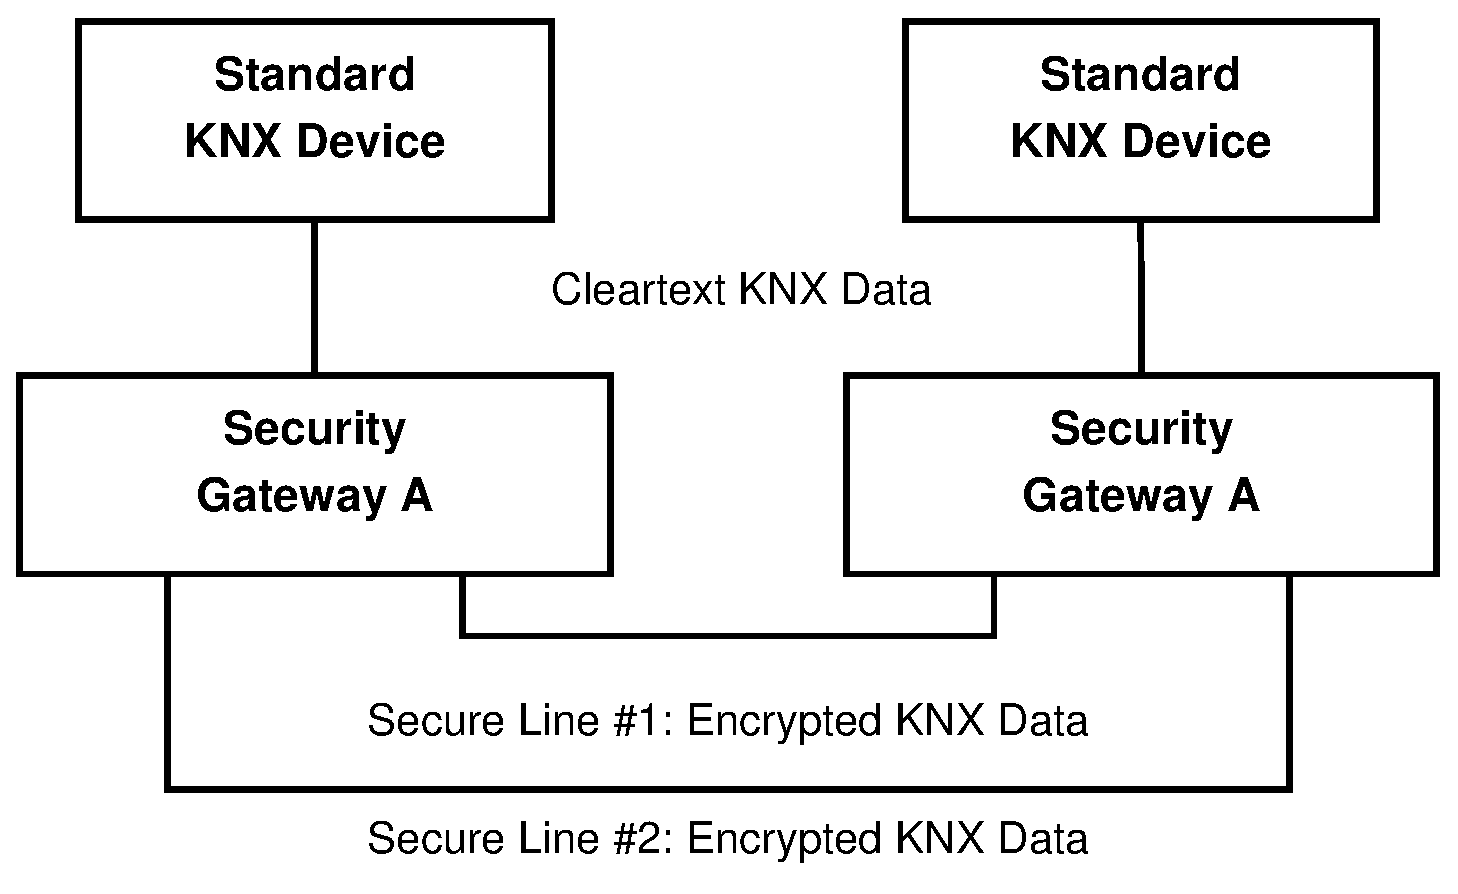
\includegraphics[width=0.8\textwidth]{figures/SecureArea.eps}
    \caption{Secure Area}
    \label{fig:secArea}
\end{figure}
\\
\\
A straightforward solution to this problem would be to wrap every datagram which enters the secured KNX network via a security gateway into a new, properly secured
broadcast datagram, and delivering this new package to the secured KNX network. Then, the package would be available to all other security gateways, which
will unwrap it and forward the resulting inner datagram to its unsecured KNX line. If the destination address (group or individual) of the actual payload
is assigned to a device connected
to the unsecured KNX network, the device holding this individual- or group-address will recognize it and the package will reach its destination. 
Otherwise it will simply be discarded.
\\
A serious constraint rising from this broadcast approach is that a single,
global network key must be used, because every security gateway must be able to decrypt and check every package which it receives on it's secured lines,
even if it does not serve as gateway to the wanted group address. 
The key of course can be renegotiated among the security gateways at every time, but this approach is considered
unsafe because an attacker can target \textit{any} of the security gateways constituting the secure network. An adversary breaking one single device gains
access to the network traffic of all devices. This could be achieved by physical access to any of the security gateways, for example by reading out the
memory of the device, and thus obtaining the globally used network key. This way, the network traffic can be decrypted by the adversary as long as no new
key is renegotiated. Another problem is that multi-party key negotiation is a costly task if a public-private key scheme
is to be used: as shown in figures \ref{fig:dh1} and \ref{fig:dh2}, a lot of messages have to be exchanged before actual an encryption can be done. 
\\
\\
To encounter this problems, different keys must be used, thus achieving pairwise end-to-end encryption between all devices. 
%This way it is also possible to achieve different security levels, depending on the function a 
%particular unsecured KNX device fulfills. It would be possible, for example, to distinguish between 'normal' gateways and 'hardened'
%gateways which are specially guarded against physical access, for example by applying physical intrusion detection. Thus,
%the risk of breaking the whole system is reduced, because breaking a device in one security level does not affect the security of the devices with other
%security levels.
%So, for breaking all $n$ security levels of a system, at least $n$ devices, all belonging to different levels must be broken.
%As a motivating example, imagine a setup which consists of window controls in an upper floor, and door controls in the
%base level. Obviously, the security constraints for the latter one would be higher. By using normal devices for window control, and hardened devices for
%door control, a security firewall can be deployed, thus containing the damage an adversary can do to the whole system.
Figure \ref{fig:firewall} shows the logical connections within an KNX network using end-to-end encryption. An 
attack of node $A$ can only compromise keys known to the device, thus effectively separating communication between the nodes $B$, $C$, and $D$ from
the attacker. 
\begin{figure}
    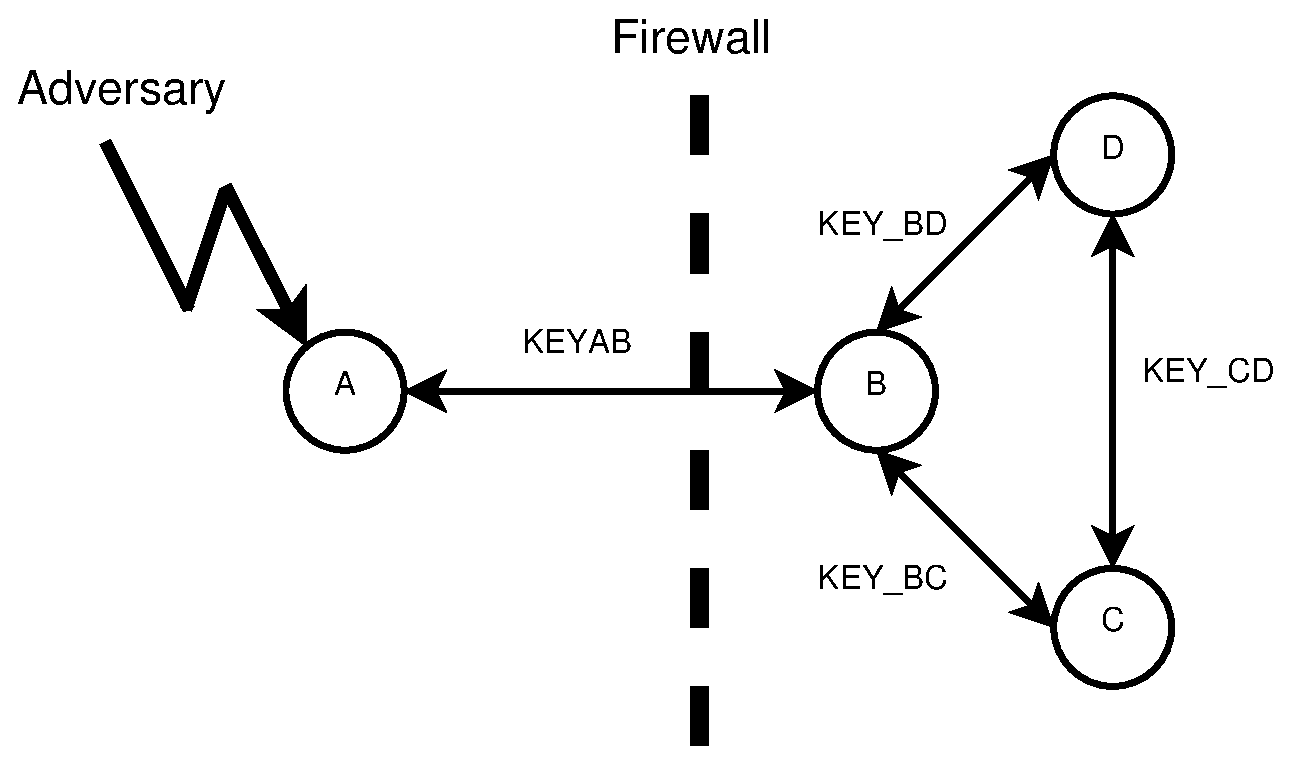
\includegraphics[width=0.8\textwidth]{figures/firewall2.eps}
% % Graphic for TeX using PGF
% Title: /home/hglanzer/ownCloud/Diplomarbeit/MasterThesisTemplate/figures/firewall.dia
% Creator: Dia v0.97.2
% CreationDate: Fri Dec  5 19:14:47 2014
% For: hglanzer
% \usepackage{tikz}
% The following commands are not supported in PSTricks at present
% We define them conditionally, so when they are implemented,
% this pgf file will use them.
\ifx\du\undefined
  \newlength{\du}
\fi
\setlength{\du}{15\unitlength}
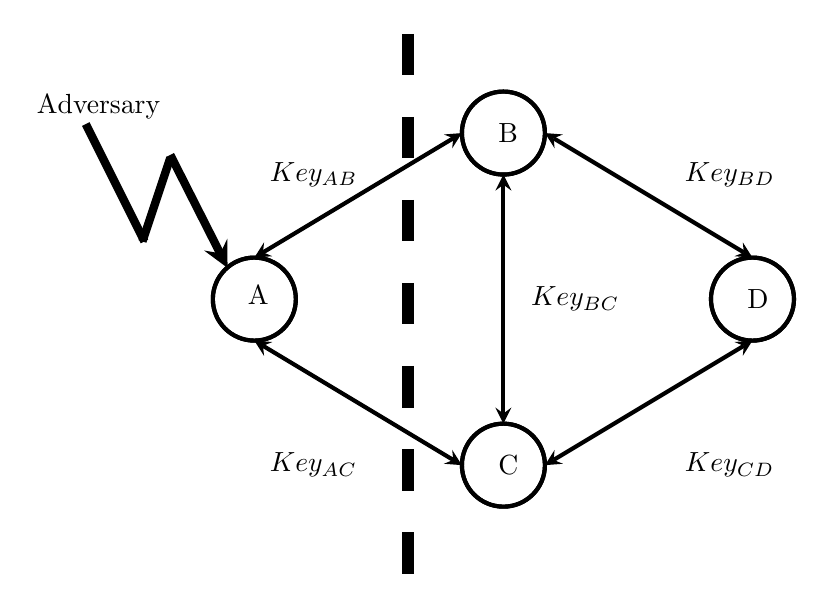
\begin{tikzpicture}
\pgftransformxscale{1.000000}
\pgftransformyscale{-1.000000}
\definecolor{dialinecolor}{rgb}{0.000000, 0.000000, 0.000000}
\pgfsetstrokecolor{dialinecolor}
\definecolor{dialinecolor}{rgb}{1.000000, 1.000000, 1.000000}
\pgfsetfillcolor{dialinecolor}
\pgfsetlinewidth{0.100000\du}
\pgfsetdash{}{0pt}
\pgfsetdash{}{0pt}
\pgfsetbuttcap
\pgfsetmiterjoin
\pgfsetlinewidth{0.100000\du}
\pgfsetbuttcap
\pgfsetmiterjoin
\pgfsetdash{}{0pt}
\definecolor{dialinecolor}{rgb}{1.000000, 1.000000, 1.000000}
\pgfsetfillcolor{dialinecolor}
\pgfpathellipse{\pgfpoint{12.000000\du}{5.000000\du}}{\pgfpoint{1.000000\du}{0\du}}{\pgfpoint{0\du}{1.000000\du}}
\pgfusepath{fill}
\definecolor{dialinecolor}{rgb}{0.000000, 0.000000, 0.000000}
\pgfsetstrokecolor{dialinecolor}
\pgfpathellipse{\pgfpoint{12.000000\du}{5.000000\du}}{\pgfpoint{1.000000\du}{0\du}}{\pgfpoint{0\du}{1.000000\du}}
\pgfusepath{stroke}
\pgfsetbuttcap
\pgfsetmiterjoin
\pgfsetdash{}{0pt}
\definecolor{dialinecolor}{rgb}{0.000000, 0.000000, 0.000000}
\pgfsetstrokecolor{dialinecolor}
\pgfpathellipse{\pgfpoint{12.000000\du}{5.000000\du}}{\pgfpoint{1.000000\du}{0\du}}{\pgfpoint{0\du}{1.000000\du}}
\pgfusepath{stroke}
\pgfsetlinewidth{0.100000\du}
\pgfsetdash{}{0pt}
\pgfsetdash{}{0pt}
\pgfsetbuttcap
\pgfsetmiterjoin
\pgfsetlinewidth{0.100000\du}
\pgfsetbuttcap
\pgfsetmiterjoin
\pgfsetdash{}{0pt}
\definecolor{dialinecolor}{rgb}{1.000000, 1.000000, 1.000000}
\pgfsetfillcolor{dialinecolor}
\pgfpathellipse{\pgfpoint{18.000000\du}{1.000000\du}}{\pgfpoint{1.000000\du}{0\du}}{\pgfpoint{0\du}{1.000000\du}}
\pgfusepath{fill}
\definecolor{dialinecolor}{rgb}{0.000000, 0.000000, 0.000000}
\pgfsetstrokecolor{dialinecolor}
\pgfpathellipse{\pgfpoint{18.000000\du}{1.000000\du}}{\pgfpoint{1.000000\du}{0\du}}{\pgfpoint{0\du}{1.000000\du}}
\pgfusepath{stroke}
\pgfsetbuttcap
\pgfsetmiterjoin
\pgfsetdash{}{0pt}
\definecolor{dialinecolor}{rgb}{0.000000, 0.000000, 0.000000}
\pgfsetstrokecolor{dialinecolor}
\pgfpathellipse{\pgfpoint{18.000000\du}{1.000000\du}}{\pgfpoint{1.000000\du}{0\du}}{\pgfpoint{0\du}{1.000000\du}}
\pgfusepath{stroke}
\pgfsetlinewidth{0.100000\du}
\pgfsetdash{}{0pt}
\pgfsetdash{}{0pt}
\pgfsetbuttcap
\pgfsetmiterjoin
\pgfsetlinewidth{0.100000\du}
\pgfsetbuttcap
\pgfsetmiterjoin
\pgfsetdash{}{0pt}
\definecolor{dialinecolor}{rgb}{1.000000, 1.000000, 1.000000}
\pgfsetfillcolor{dialinecolor}
\pgfpathellipse{\pgfpoint{18.000000\du}{9.000000\du}}{\pgfpoint{1.000000\du}{0\du}}{\pgfpoint{0\du}{1.000000\du}}
\pgfusepath{fill}
\definecolor{dialinecolor}{rgb}{0.000000, 0.000000, 0.000000}
\pgfsetstrokecolor{dialinecolor}
\pgfpathellipse{\pgfpoint{18.000000\du}{9.000000\du}}{\pgfpoint{1.000000\du}{0\du}}{\pgfpoint{0\du}{1.000000\du}}
\pgfusepath{stroke}
\pgfsetbuttcap
\pgfsetmiterjoin
\pgfsetdash{}{0pt}
\definecolor{dialinecolor}{rgb}{0.000000, 0.000000, 0.000000}
\pgfsetstrokecolor{dialinecolor}
\pgfpathellipse{\pgfpoint{18.000000\du}{9.000000\du}}{\pgfpoint{1.000000\du}{0\du}}{\pgfpoint{0\du}{1.000000\du}}
\pgfusepath{stroke}
\pgfsetlinewidth{0.100000\du}
\pgfsetdash{}{0pt}
\pgfsetdash{}{0pt}
\pgfsetbuttcap
\pgfsetmiterjoin
\pgfsetlinewidth{0.100000\du}
\pgfsetbuttcap
\pgfsetmiterjoin
\pgfsetdash{}{0pt}
\definecolor{dialinecolor}{rgb}{1.000000, 1.000000, 1.000000}
\pgfsetfillcolor{dialinecolor}
\pgfpathellipse{\pgfpoint{24.000000\du}{5.000000\du}}{\pgfpoint{1.000000\du}{0\du}}{\pgfpoint{0\du}{1.000000\du}}
\pgfusepath{fill}
\definecolor{dialinecolor}{rgb}{0.000000, 0.000000, 0.000000}
\pgfsetstrokecolor{dialinecolor}
\pgfpathellipse{\pgfpoint{24.000000\du}{5.000000\du}}{\pgfpoint{1.000000\du}{0\du}}{\pgfpoint{0\du}{1.000000\du}}
\pgfusepath{stroke}
\pgfsetbuttcap
\pgfsetmiterjoin
\pgfsetdash{}{0pt}
\definecolor{dialinecolor}{rgb}{0.000000, 0.000000, 0.000000}
\pgfsetstrokecolor{dialinecolor}
\pgfpathellipse{\pgfpoint{24.000000\du}{5.000000\du}}{\pgfpoint{1.000000\du}{0\du}}{\pgfpoint{0\du}{1.000000\du}}
\pgfusepath{stroke}
\pgfsetlinewidth{0.100000\du}
\pgfsetdash{}{0pt}
\pgfsetdash{}{0pt}
\pgfsetbuttcap
{
\definecolor{dialinecolor}{rgb}{0.000000, 0.000000, 0.000000}
\pgfsetfillcolor{dialinecolor}
% was here!!!
\pgfsetarrowsstart{stealth}
\pgfsetarrowsend{stealth}
\definecolor{dialinecolor}{rgb}{0.000000, 0.000000, 0.000000}
\pgfsetstrokecolor{dialinecolor}
\draw (17.000000\du,1.000000\du)--(12.000000\du,4.000000\du);
}
\pgfsetlinewidth{0.100000\du}
\pgfsetdash{}{0pt}
\pgfsetdash{}{0pt}
\pgfsetbuttcap
{
\definecolor{dialinecolor}{rgb}{0.000000, 0.000000, 0.000000}
\pgfsetfillcolor{dialinecolor}
% was here!!!
\pgfsetarrowsstart{stealth}
\pgfsetarrowsend{stealth}
\definecolor{dialinecolor}{rgb}{0.000000, 0.000000, 0.000000}
\pgfsetstrokecolor{dialinecolor}
\draw (12.000000\du,6.000000\du)--(17.000000\du,9.000000\du);
}
\pgfsetlinewidth{0.100000\du}
\pgfsetdash{}{0pt}
\pgfsetdash{}{0pt}
\pgfsetbuttcap
{
\definecolor{dialinecolor}{rgb}{0.000000, 0.000000, 0.000000}
\pgfsetfillcolor{dialinecolor}
% was here!!!
\pgfsetarrowsstart{stealth}
\pgfsetarrowsend{stealth}
\definecolor{dialinecolor}{rgb}{0.000000, 0.000000, 0.000000}
\pgfsetstrokecolor{dialinecolor}
\draw (19.000000\du,9.000000\du)--(24.000000\du,6.000000\du);
}
\pgfsetlinewidth{0.100000\du}
\pgfsetdash{}{0pt}
\pgfsetdash{}{0pt}
\pgfsetbuttcap
{
\definecolor{dialinecolor}{rgb}{0.000000, 0.000000, 0.000000}
\pgfsetfillcolor{dialinecolor}
% was here!!!
\pgfsetarrowsstart{stealth}
\pgfsetarrowsend{stealth}
\definecolor{dialinecolor}{rgb}{0.000000, 0.000000, 0.000000}
\pgfsetstrokecolor{dialinecolor}
\draw (19.000000\du,1.000000\du)--(24.000000\du,4.000000\du);
}
\pgfsetlinewidth{0.100000\du}
\pgfsetdash{}{0pt}
\pgfsetdash{}{0pt}
\pgfsetbuttcap
{
\definecolor{dialinecolor}{rgb}{0.000000, 0.000000, 0.000000}
\pgfsetfillcolor{dialinecolor}
% was here!!!
\pgfsetarrowsstart{stealth}
\pgfsetarrowsend{stealth}
\definecolor{dialinecolor}{rgb}{0.000000, 0.000000, 0.000000}
\pgfsetstrokecolor{dialinecolor}
\draw (18.000000\du,2.000000\du)--(18.000000\du,8.000000\du);
}
\pgfsetlinewidth{0.300000\du}
\pgfsetdash{{1.000000\du}{1.000000\du}}{0\du}
\pgfsetdash{{1.000000\du}{1.000000\du}}{0\du}
\pgfsetbuttcap
{
\definecolor{dialinecolor}{rgb}{0.000000, 0.000000, 0.000000}
\pgfsetfillcolor{dialinecolor}
% was here!!!
\definecolor{dialinecolor}{rgb}{0.000000, 0.000000, 0.000000}
\pgfsetstrokecolor{dialinecolor}
\draw (15.707107\du,-1.388909\du)--(15.707107\du,11.611091\du);
}
% setfont left to latex
\definecolor{dialinecolor}{rgb}{0.000000, 0.000000, 0.000000}
\pgfsetstrokecolor{dialinecolor}
\node[anchor=west] at (18.292893\du,5.000000\du){$Key_{BC}$};
% setfont left to latex
\definecolor{dialinecolor}{rgb}{0.000000, 0.000000, 0.000000}
\pgfsetstrokecolor{dialinecolor}
\node[anchor=west] at (11.469670\du,4.893934\du){A};
% setfont left to latex
\definecolor{dialinecolor}{rgb}{0.000000, 0.000000, 0.000000}
\pgfsetstrokecolor{dialinecolor}
\node[anchor=west] at (17.505025\du,1.000000\du){B};
% setfont left to latex
\definecolor{dialinecolor}{rgb}{0.000000, 0.000000, 0.000000}
\pgfsetstrokecolor{dialinecolor}
\node[anchor=west] at (17.505025\du,9.000000\du){C};
% setfont left to latex
\definecolor{dialinecolor}{rgb}{0.000000, 0.000000, 0.000000}
\pgfsetstrokecolor{dialinecolor}
\node[anchor=west] at (23.505025\du,5.000000\du){D};
% setfont left to latex
\definecolor{dialinecolor}{rgb}{0.000000, 0.000000, 0.000000}
\pgfsetstrokecolor{dialinecolor}
\node[anchor=west] at (12.000000\du,2.000000\du){$Key_{AB}$};
% setfont left to latex
\definecolor{dialinecolor}{rgb}{0.000000, 0.000000, 0.000000}
\pgfsetstrokecolor{dialinecolor}
\node[anchor=west] at (12.000000\du,9.000000\du){$Key_{AC}$};
% setfont left to latex
\definecolor{dialinecolor}{rgb}{0.000000, 0.000000, 0.000000}
\pgfsetstrokecolor{dialinecolor}
\node[anchor=west] at (22.000000\du,2.000000\du){$Key_{BD}$};
% setfont left to latex
\definecolor{dialinecolor}{rgb}{0.000000, 0.000000, 0.000000}
\pgfsetstrokecolor{dialinecolor}
\node[anchor=west] at (22.000000\du,9.000000\du){$Key_{CD}$};
% setfont left to latex
\definecolor{dialinecolor}{rgb}{0.000000, 0.000000, 0.000000}
\pgfsetstrokecolor{dialinecolor}
\node[anchor=west] at (14.000000\du,9.000000\du){};
\pgfsetlinewidth{0.200000\du}
\pgfsetdash{}{0pt}
\pgfsetdash{}{0pt}
\pgfsetbuttcap
{
\definecolor{dialinecolor}{rgb}{0.000000, 0.000000, 0.000000}
\pgfsetfillcolor{dialinecolor}
% was here!!!
\definecolor{dialinecolor}{rgb}{0.000000, 0.000000, 0.000000}
\pgfsetstrokecolor{dialinecolor}
\draw (7.939094\du,0.782827\du)--(9.353307\du,3.611255\du);
}
\pgfsetlinewidth{0.200000\du}
\pgfsetdash{}{0pt}
\pgfsetdash{}{0pt}
\pgfsetbuttcap
{
\definecolor{dialinecolor}{rgb}{0.000000, 0.000000, 0.000000}
\pgfsetfillcolor{dialinecolor}
% was here!!!
\definecolor{dialinecolor}{rgb}{0.000000, 0.000000, 0.000000}
\pgfsetstrokecolor{dialinecolor}
\draw (9.303307\du,3.611255\du)--(9.975059\du,1.596000\du);
}
\pgfsetlinewidth{0.200000\du}
\pgfsetdash{}{0pt}
\pgfsetdash{}{0pt}
\pgfsetbuttcap
{
\definecolor{dialinecolor}{rgb}{0.000000, 0.000000, 0.000000}
\pgfsetfillcolor{dialinecolor}
% was here!!!
\pgfsetarrowsend{stealth}
\definecolor{dialinecolor}{rgb}{0.000000, 0.000000, 0.000000}
\pgfsetstrokecolor{dialinecolor}
\draw (9.975059\du,1.525290\du)--(11.353917\du,4.247651\du);
}
% setfont left to latex
\definecolor{dialinecolor}{rgb}{0.000000, 0.000000, 0.000000}
\pgfsetstrokecolor{dialinecolor}
\node[anchor=west] at (6.439525\du,0.358563\du){Adversary};
\end{tikzpicture}

 \caption{Firewall}
 \label{fig:firewall}
\end{figure}
\\
\\
As stated above, to be able to use different keys every security gateway has to know how to reach a given address so that the data can be encrypted
exclusively for the responsible gateway. The solution to this problem is to maintain some kind of routing table, mapping group and individual addresses of unsecured
KNX devices to individual addresses of responsible security gateways. Additionally, this table must hold the key that will be used for encryption.
Such a routing table can be built statically at setup time, with the obvious disadvantage
that the exact topology of the to be applied network has to be known in advance, thus reducing the flexibility. Here, every security gateway holds a static 
table which consists of mappings between individual- or group addresses of unsecured KNX devices and individual addresses of security gateways at the border
between the secured and the unsecured KNX network, as well as all keys used for the particular security level the gateway belongs to.
This table would be generated once, after the topology of the network has been fixed, must be equipped with the proper keys and can then
be copied to the security gateways constituting the secured KNX area. New security gateways can be deployed as long as they only introduce sending 
unsecured KNX devices, whose recipients are already mapped, known group addresses. A new group address, introduced by a newly installed device behind
an already existing security gateway, will not be reachable, simply because the routing information is not available. 
Another disadvantage is that the deployment of new
security gateways, connecting devices with new or already known group addresses, is impossible as the individual address of the new gateway - which of
course must be unique - is unknown to the existing setup, thus making the new unsecured KNX devices unreachable.
\\
To tackle this problem, another approach would be to build this mapping table dynamically. Therefore, every security gateway must periodically poll
on it's unsecured lines for KNX devices(FIXME: HOW? analog zu ETS group address polling), thus populating a list of reachable KNX devices. Whenever a 
device wants to send data to a group address, it has to do a lookup first to obtain the individual addresses of the responsible security gateways: the lookup
must contain the wanted group address, as well as the senders public key.
Every 
gateway which finds the wanted group address in its group list must reply with an according message to the requester, thus announcing that it is responsible
for delivering data to the wanted group address, and must also publish it's own public key, thus allowing pairwise end-to-end encryption.
The original requester must wait for a short time for replies, possibly retransmitting the request in case
of no responses, and can then transmit the encrypted package to all responsible gateways, if any, one at a time. This procedure requires no a priori knowledge of
the network topology, so security gateways can be added to the network as well as unsecured KNX devices behind new or existing gateways at any time. This
flexibility of course has to be purchased with increased complexity as well as additional traffic induced into the network.
\\
\\
As a middle course it would be viable to generate the reachable group address list whenever a new security gateway is added to the network,
and handle discovery of this group addresses as described
above. This allows to deploy new security gateways with connected unsecured devices, thus achieving a comprise between flexibility and complexity.


\subsection{Security Related Architectural Overview}
While it would be possible to use a centralized concept, no trusted on-line party is used in this work. This decentralized setup is used
to simplify the setup. A centralized approach would need fall-back key servers
which inherit the task of generating and distributing keys and parameters in case of a master key server failure. Otherwise, the network would suffer from a
single point of failure in case no such fall-back mechanism is applied, an assumption that would clearly disqualify the design as highly available.	 
\\
\\
To provide authenticity, all datagrams passing the secured KNX network must contain a \gls{mac2} to prevent modification of them(i.e. to guard against active
adversaries). This \gls{mac2} must be combined with a counter value to avoid replay attacks. The counter must be strictly monotonically increasing and must not overflow.
The counter can be seen as initialization vector that prevents the mapping of same cleartext messages to same ciphertext messages under the same
encryption key.
To guard against passive adversaries, i.e. eavesdropping, all datagrams carrying KNX application data must be encrypted. These are all datagrams coming from outside of the
secured area, originating from an unsecured KNX device. As explained above, these packages will be encrypted end-to-end, with unique asymmetric keys between
each two communication partners.
Additionally, all discovery messages generated by security gateways will be encrypted too. Although these datagrams don't contain KNX data per se, they allow
a listening adversary to learn the topology of the network, knowledge which can be valuable for developing an attack strategy, as well as generating meta data.
For example, if an attacker learns that a particular security gateway is responsible for only one group address and further gets knowledge that this 
group address is responsible for switching a light (i.e. by visual observation), the attacker afterwards may be able to derive a personal profile just by seeing
packages for this group address, although the datagrams are encrypted. If the discovery messages are encrypted too the adversary doesn't know how many
group addresses are behind the gateway, and it will be harder to derive personal profiles or to gather knowledge of the network topology.

\subsection{Redundancy Related Architectural Overview}

To achieve a higher level of availability, all components that are needed to provide a specific service must exist multiple times. 
\\
\\
Whenever a KNX package is
generated by a device on an unsecured line (called client), the connected security gateway will read, duplicate and encapsulate it into another KNX frame 
and then send over booth lines. If booth lines are available, i.e. there is, for example, no shortcut, a receiving security gateway will receive 2
different KNX frames encapsulating the same
payload, which itself is the KNX frame generated by the KNX client device in the first place. One message must be discarded to avoid duplicates. This is 
achieved with a monotonically increasing counter that also guards against replay attacks: whenever a package, generated by a client, enters the
network, a counter for outgoing packages is incremented
which must be sent along the duplicated packages so that the receiving side can discard one of the 2 packages. This counter must be
unambiguous for every source/destination address tuple of the origin cleartext message. The receiving side must maintain a counter for incoming packets, 
also uniquely identified by source and destination address. If booth lines are available, one message will be handled first and trigger an incrementation of the
corresponding source/destination counter. The duplicated message, which is handled after that, can safely be discarded because the corresponding counter
value will be less than the saved value. Nevertheless which package from which secure line is forwarded to the unsecured line, each line must acknowledge
every received package: this is done by generating a special acknowledge frame which is sent back to the sending gateway. The payload of this package must
allow the sending gateway to unambiguously identify the acknowledged package, i.e. it must bear source and destination address of the package generated
by the client, as well as the used counter value. As a consequence, these acknowledgement frames must be encrypted and authenticated as well.
If no acknowledgement frame is received within time $t_{ACK}$, a retransmission is done on booth lines. This retransmission simply re-submits the same
package with the same counter value again. Regarding the security this is no problem because a passive attacker can not learn anything from such a repeated
package.


\subsection{Operational Constrains}

The introduction of encapsulating security gateways implicates that some timing constraints, defined by KNX, cannot be met:

\begin{itemize}
 \item Acknowledge frames, as defined in KNX and introduced in chapter \ref{ch:knx}, cannot be guaranteed to be delivered within the specified deadlines: whenever
 a new KNX datagram is generated by a client, at first the discovery phase has to occur. Only after that the to-acknowledged frame is sent. So there are
 multiple delays introduced, stalling the delivery: the first delay is caused by sending of the discovery package.
 After that, a second delay occurs because the security gateway must wait for the discovery response(s), possibly retransmitting the discovery request
 in case of a timeout. After receiving discovery responses, the third delay is caused by sending the actual, encapsulated
 client package to the responsible security gateway(s), which then must check the datagram, unpack it and forward it on it's unsecured line.
 Only after that, all addressed, unsecured clients would be able to acknowledge the received frames
 to their local security gateways,
 which must forwarded the acknowledgement frame to the origin security gateway, causing another delay. Finally, the acknowledgement frame must be forwarded to the sender of
 the origin data frame, causing another delay.
 These delays will always occur, and most of them cannot be restricted, thus destroying the tight timing constraints for acknowledgement frames, as defined
 by the KNX standard. This
 will most likely result in multiple retransmissions of the same KNX packages
 by the client because the client's timer will generate a timeout. The only way to solve this is to immediately acknowledge a client frame by the security
 gateway that it is connected to. On the receiving side, the client will generate an acknowledge
 frame, which must be discarded by it's security gateway.
 \item Similar arguments avoid the processing of Poll-Data Frames. Here, event more stringent timing constraints are to be met, see chapter \ref{ch:knx}. 
\end{itemize}

\subsection{Operation states FIXME}

synchronization

joininig

discovery

data

\subsection{Key Management}

The previous statements imply that 3 different kind of keys must be used:

\begin{itemize}
 \item First, a long-term key known to all security gateways is used. As already stated, this key must be copied to every device at setup time. 
This pre-shared key $k_{psk}$ is used for symmetric encryption and serves 2 different purposes: first, it is used to authenticate the global counter
value sent to  new devices which want to join the network, as well for devices that have lost their synchronization (i.e. that have been unavailable for some
 time). Additionally, this key $k_{psk}$ is used to encrypt another symmetric key $k_{global}$, which every device must obtain in the joining phase to be 
 able to take part in the discovery procedures. 
 \item $k_{global}$ is used to authenticate and encrypt locally generated and decrypt received discovery requests, as well as to authenticate and encrypt
 locally generated discovery responses and decrypt received ones. This discovery service datagrams securely transport the third type of keys:
 \item Asymmetric keys are used for end-to-end encryption of the actual data packages between 2 security gateways.
\end{itemize}

\subsection{High Level Cryptography Library}

\subsubsection{OpenSSL}

\begin{itemize}
 \item install libssl, libssl-dev
\end{itemize}

\subsubsection{Crypto++}
\begin{itemize}
 \item install  libcrypto++9
\end{itemize}